\documentclass[14pt,a4paper]{extarticle}

\usepackage{cmap}
\usepackage[T2A]{fontenc}
\usepackage[utf8]{inputenc}
\usepackage[russian]{babel}
\usepackage{newtxtext,newtxmath}

\usepackage{amsmath}
\usepackage{geometry}
\usepackage{setspace}
\usepackage{indentfirst}
\usepackage{graphicx}
\usepackage{array}
\usepackage{caption}
\usepackage{booktabs}
\usepackage{siunitx}
\sisetup{output-decimal-marker={,}, separate-uncertainty, per-mode=symbol}
\DeclareSIUnit\joule{\text{Дж}}
\DeclareSIUnit\kelvin{\text{К}}
\DeclareSIUnit\newton{\text{Н}}
\DeclareSIUnit\metre{\text{м}}
\DeclareSIUnit\pascal{\text{Па}}
\captionsetup[table]{labelsep=endash, justification=raggedright, singlelinecheck=false}
\captionsetup[figure]{labelsep=endash}
\usepackage{pgfplots}
\pgfplotsset{compat=1.18}

\geometry{left=30mm, right=10mm, top=20mm, bottom=20mm}
\onehalfspacing
\setlength{\parindent}{1.25cm}
\pagestyle{plain}

\begin{document}

\begin{titlepage}
\begin{center}
\onehalfspacing
Белорусский государственный университет\\
Факультет радиофизики и компьютерных технологий

\vspace{4cm}

\textbf{ОТЧЁТ}\\
по лабораторной работе №4\\[0.3cm]
\textbf{«Интерферометр Рэлея»}

\vspace{4cm}

\begin{flushright}
\begin{tabular}{@{}p{7.5cm}@{}}
\raggedright
Выполнил:\\
студент 2 курса 8 группы\\
Нацевский М. А.\\
Преподаватель:\\
Трухан С. В.\\
\end{tabular}
\end{flushright}

\vfill
Минск, 2026
\end{center}
\end{titlepage}
\setcounter{page}{2}

\section*{Цель работы}

Изучить устройство и принцип работы интерферометра Рэлея. Измерить поляризуемость молекул воздуха.

\section*{Краткая теория}

\begin{figure}[h]
  \begin{center}
    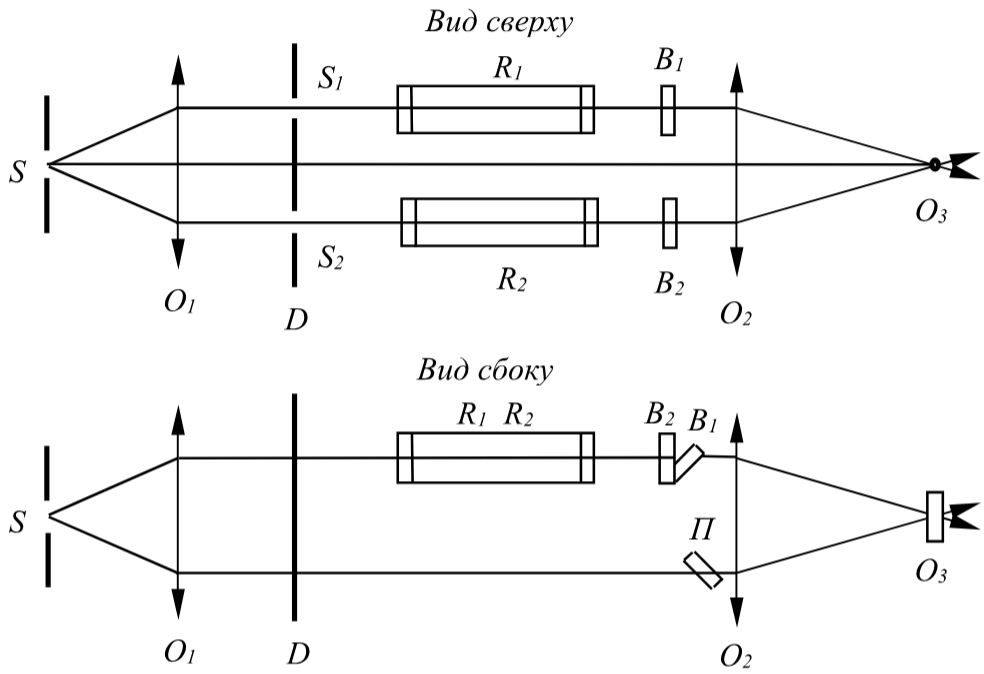
\includegraphics[width=0.75\textwidth]{scheme.png}
  \end{center}
  \caption{Схема интерферометра ИТР-1 в двух разрезах}\label{fig:}
\end{figure}

Узкая щель $S$, расположенная в фокальной плоскости объектива $O_1$, вместе с ним образует коллиматор. Параллельный пучок лучей проходит диафрагму $D$ с двумя щелями $S_1$ и $S_2$, параллельными $S$, и две одинаковые кюветы $R_1$ и $R_2$ с исследуемыми газами или жидкостями. В результате интерференции света, дифрагировавшего на щелях $S_1$ и $S_2$, в фокальной плоскости объектива $O_2$ образуется система изображений щели $S$ (максимумы разных порядков).

Размещение кювет требует большого расстояния между $S_1$ и $S_2$, поэтому полосы расположены тесно, а из"=за узости щелей яркость картины невелика. Увеличение нужно только в направлении, перпендикулярном полосам, поэтому используется цилиндрический окуляр $O_3$ "--- тонкая стеклянная палочка, ось которой параллельна полосам. Картина при этом значительно ярче, чем при сферическом окуляре.

Кюветы занимают лишь верхнюю часть пучка. Свет от $S_1$ и $S_2$, прошедший ниже кювет, даёт вторую систему полос с тем же периодом, которая служит шкалой отсчёта. С помощью стеклянной пластинки $\Pi$ её смещают по вертикали так, чтобы она примыкала к главной системе; линией раздела служит край пластинки. Глаз способен заметить смещение порядка $1/40$ полосы. Случайные смещения элементов системы действуют на обе системы полос одинаково и потому мало влияют на результат.

Смещение главной системы полос относительно шкалы определяет оптическую разность хода $\Delta$ между лучами, прошедшими через кюветы $R_1$ и $R_2$, а значит, и разность показателей преломления $\Delta n = n_1 - n_2$:
\begin{equation}
    \Delta = n_1 L - n_2 L = (n_1 - n_2)L = \Delta n\, L,
\end{equation}
где $L$ "--- длина кювет.
\section*{Экспериментальная часть}

При одинаковом давлении в кюветах, равном атмосферному, было определено значение $m_0 = 277{,}5$ дел. по микровинту.
Дальнейшие измерения $m$, $\Delta m$ производились со ступенчатым увеличением давления $P$ в одной из кювет.
Для каждой разности давлений компенсация сдвига полос производилась 2 раза, за результат принято среднее значение $m_{\text{ср}}$.

На практике удобнее не считать полосы, а компенсировать разность хода. Свет, выходящий из кювет, проходит через тонкие стеклянные пластинки $B_1$ и $B_2$: одна неподвижна, а другая (например, $B_1$) может поворачиваться вокруг горизонтальной оси, плавно изменяя оптическую длину пути луча, выходящего из $S_1$. Компенсатор калибруется, и по углу поворота пластинки по калибровочному графику определяется оптическая разность хода $\Delta$.
\begin{table}[htbp]
\caption{Результаты измерений}
\label{tab:rt}
\centering
\small
\setlength{\tabcolsep}{4pt}
\begin{tabular}{
S[table-format=2.0]
S[table-format=4.0]
S[table-format=4.0]
S[table-format=4.0]
S[table-format=4.1]
S[table-format=4.1]
S[table-format=2.1]
S[table-format=2.1]
}
\toprule
{$\Delta P$, см в.\,ст.} & {$\Delta P$, Па} & {$m_1$} & {$m_2$} & {$m_{\text{ср}}$} & {$\Delta m$} & {$\Delta$, $10^{-4}$ см} & {$\Delta n$, $10^{-6}$} \\
\midrule
0 & 0 & 277 & 278 & 277,5 & 0 & 0 & 0 \\
5 & 490 & 418 & 370 & 394 & 116,5 & 2 & 2 \\
10 & 981 & 424 & 416 & 420 & 142,5 & 2,1 & 2,1 \\
15 & 1471 & 529 & 520 & 524,5 & 247 & 4,6 & 4,6 \\
20 & 1961 & 613 & 547 & 580 & 302,5 & 5,4 & 5,4 \\
25 & 2452 & 617 & 735 & 676 & 398,5 & 7,5 & 7,5 \\
30 & 2942 & 867 & 844 & 855,5 & 578 & 10,7 & 10,7 \\
35 & 3432 & 861 & 835 & 848 & 570,5 & 10,6 & 10,6 \\
40 & 3923 & 1013 & 987 & 1000 & 722,5 & 13,4 & 13,4 \\
50 & 4903 & 1117 & 1065 & 1091 & 813,5 & 15,6 & 15,6 \\
77 & 7551 & 1543 & 1600 & 1571,5 & 1294 & 24,6 & 24,6 \\
87 & 8532 & 1853 & 1810 & 1831,5 & 1554 & 28,5 & 28,5 \\
\bottomrule
\end{tabular}
\end{table}

При измерениях температура воздуха составляла $\SI{21}{\celsius}$, или $T = \SI{294,15}{\kelvin}$.

\section*{Обработка экспериментальных данных}

С помощью градуировочного графика для всех значений $\Delta m$ были найдены соответствующие значения оптической разности хода $\Delta$.
Значения $\Delta n$ были найдены по формуле $\Delta n = \Delta / L$, где $L = \SI{1}{\metre}$ --- длина кювет.

Зависимость $\Delta n = f(\Delta P)$ приведена на рис.~\ref{fig:dn}. Угловой коэффициент $\beta$ в зависимости $\Delta n = \beta\,\Delta P$ найден методом наименьших квадратов:
\[
\beta = \frac{N\sum \Delta P_i \Delta n_i - \sum \Delta P_i \sum \Delta n_i}{N\sum \Delta P_i^2 - \left(\sum \Delta P_i\right)^2}
= \SI{3,34e-9}{\square\metre\per\newton}.
\]

\begin{figure}[htbp]
\centering
\begin{tikzpicture}
\begin{axis}[
  width=0.9\textwidth, height=8cm,
  xlabel={$\Delta P$, Па}, ylabel={$\Delta n \cdot 10^{-6}$},
  grid=major, xmin=0, ymin=0, legend pos=north west
]
\addplot[only marks, mark=*, blue] coordinates {
(0,0) (490,2) (981,2.1) (1471,4.6) (1961,5.4) (2452,7.5)
(2942,10.7) (3432,10.6) (3923,13.4) (4903,15.6) (7551,24.6) (8532,28.5)
};
\addplot[red, thick, domain=0:8700] {0.0033397*x - 0.3365};
\legend{Эксперимент, МНК}
\end{axis}
\end{tikzpicture}
\caption{Зависимость $\Delta n$ от $\Delta P$}
\label{fig:dn}
\end{figure}

Поляризуемость воздуха:
\[
\alpha = 2kT\beta = A T \beta = \SI{2,762e-23}{\joule\per\kelvin} \cdot \SI{294,15}{\kelvin} \cdot \SI{3,34e-9}{\square\metre\per\newton} \approx \SI{2,71e-29}{\cubic\metre}.
\]
Погрешность, найденная по остаточной дисперсии МНК, составляет $\SI{0,04e-29}{\cubic\metre}$.

\section*{Вывод}

Изучено устройство и принцип работы интерферометра Рэлея. Экспериментально подтверждена линейная зависимость показателя преломления воздуха от давления. Поляризуемость молекул воздуха составила $\alpha = (2{,}71 \pm 0{,}04)\cdot 10^{-29}$~м$^3$, что по порядку величины согласуется с ожидаемым значением.

\end{document}
